\chapter{Soluciones\\Álgebra  II -- Año 2024/1 -- FAMAF}\label{practico-2}

\begin{enumerate}[topsep=6pt, itemsep=.4cm]
\item {\it Juego Suko}. Colocar los números del $1$ al $9$ en las celdas de la siguiente tabla de modo que el número en cada círculo sea igual a la suma de las cuatro celdas adyacentes, y la suma de las celdas del mismo color sea igual al número en el círculo de igual color.

\begin{center}
  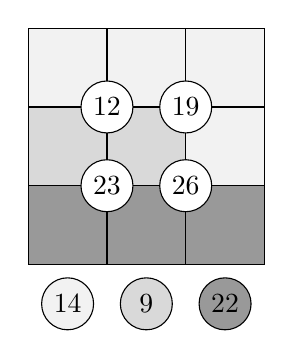
\begin{tikzpicture}
    \draw [fill=gray!10] (0,0) rectangle (1,-1); 
    \draw [fill=gray!10] (1,0) rectangle (2,-1); 
    \draw [fill=gray!10] (2,0) rectangle (3,-1); 
    \draw [fill=gray!30] (0,-1) rectangle (1,-2); 
    \draw [fill=gray!30] (1,-1) rectangle (2,-2); 
    \draw [fill=gray!10] (2,-1) rectangle (3,-2); 
    \draw [fill=gray!80] (0,-2) rectangle (1,-3); 
    \draw [fill=gray!80] (1,-2) rectangle (2,-3); 
    \draw [fill=gray!80] (2,-2) rectangle (3,-3); 
    \filldraw[fill=white](1,-1) circle (0.33);
    \filldraw[fill=white](2,-1) circle (0.33);
    \filldraw[fill=white](1,-2) circle (0.33);
    \filldraw[fill=white](2,-2) circle (0.33);
    \node at (1,-1) {12};
    \node at (2,-1) {19};
    \node at (1,-2) {23};
    \node at (2,-2) {26};
    \filldraw[fill=gray!10](0.5,-3.5) circle (0.33);
    \filldraw[fill=gray!30](1.5,-3.5) circle (0.33);
    \filldraw[fill=gray!80](2.5,-3.5) circle (0.33);
    \node at (0.5,-3.5) {14};
    \node at (1.5,-3.5) {9};
    \node at (2.5,-3.5) {22};
    
    \end{tikzpicture}
\end{center}

\rta Queremos ver que valor toma cada celda y, por lo tanto,  a cada celda le asignamos una variable:
\begin{center}
  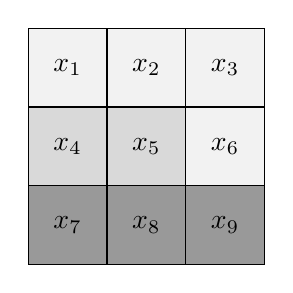
\begin{tikzpicture}
    \draw [fill=gray!10] (0,0) rectangle (1,-1); 
    \draw [fill=gray!10] (1,0) rectangle (2,-1); 
    \draw [fill=gray!10] (2,0) rectangle (3,-1); 
    \draw [fill=gray!30] (0,-1) rectangle (1,-2); 
    \draw [fill=gray!30] (1,-1) rectangle (2,-2); 
    \draw [fill=gray!10] (2,-1) rectangle (3,-2); 
    \draw [fill=gray!80] (0,-2) rectangle (1,-3); 
    \draw [fill=gray!80] (1,-2) rectangle (2,-3); 
    \draw [fill=gray!80] (2,-2) rectangle (3,-3); 
    \node at (0.5,-0.5) {$x_1$};
    \node at (1.5,-0.5) {$x_2$};
    \node at (2.5,-0.5) {$x_3$};
    \node at (0.5,-1.5) {$x_4$};
    \node at (1.5,-1.5) {$x_5$};
    \node at (2.5,-1.5) {$x_6$};
    \node at (0.5,-2.5) {$x_7$};
    \node at (1.5,-2.5) {$x_8$};
    \node at (2.5,-2.5) {$x_9$};
    \end{tikzpicture}
\end{center}
Tenemos entonces las $9$ incógnitas que debemos resolver y la información del Suko original nos dice que se deben cumplir las siguientes ecuaciones:
\begin{align}
&x_1 + x_2 +x_4 +x_5 =12,  \\
&x_2+ x_3+x_5 +x_6 = 19, \\
&x_4 +x_5 +x_7 + x_8 = 23, \\
&x_5 +x_6 +x_8 + x_9 = 26, \\
&x_4 + x_5 = 9, \\
&x_1+x_2 +x_3 +x_6 = 14, \\
&x_7+ x_8 + x_9 = 22
\end{align}


Primero vamos a tratar de resolver el sistema de ecuaciones. Podríamos plantear  la matriz ampliada del sistema y  reducir la matriz, pero en este caso va a resultar más corto trabajar con las ecuaciones directamente. Hay 9 incógnitas y 7 ecuaciones, entonces en general es razonable que queden 7 variables dependientes y 2 variables libres. Con esto en mente trataremos de despejar todo en función de las variables $x_1$ y $x_3$ (esto fue elegido arbitrariamente). 


Como $x_4 + x_5 = 9$ $\;\stackrel{(1)}{\Rightarrow}\;$ $x_1 + x_2 + 9 =12$,  es decir $x_1 + x_2  =3$ o \colorbox{green!20}{$x_2 = 3 -x_1$ ($a$)}.


Como $x_4 + x_5 = 9$ 
$\;\stackrel{(3)}{\Rightarrow}\;$ 
$9+x_7 + x_8 = 23$ 
$\;\stackrel{}{\Rightarrow}\;$
$x_7 + x_8 = 14$ 
$\;\stackrel{(7)}{\Rightarrow}\;$
$14 + x_9 = 22$ $\;\stackrel{}{\Rightarrow}\;$ \colorbox{green!20}{$x_9 = 8$ ($b$)}.

Ahora, como $x_1 + x_2 = 3$ $\;\stackrel{(6)}{\Rightarrow}\;$ $3 +x_3 +x_6 = 14$,  es decir $x_3 +x_6 = 11$ o \colorbox{green!20}{$x_6 = 11 -x_3$ ($c$)}. 

Si en la ecuación (2) reemplazamos $x_2$ y $x_6$, obtenemos
$$
19 = x_2+ x_3+x_5 +x_6 = (3 -x_1) + x_3 + x_5 +(11 -x_3) = 14 -x_1 +x_5,
$$
o \colorbox{green!20}{$x_5 = 5 +x_1$ ($d$)}.

Con todo lo que hemos averiguado hacemos reemplazos en (4):
$$
26 = x_5 +x_6 +x_8 + x_9 = ( 5 +x_1) +( 11 -x_3) +x_8 + 8 = 24 +x_1 - x_3 + x_8, 
$$ 
luego \colorbox{green!20}{$x_8 = 2 -x_1 + x_3$ ($e$)}.

De la fórmula (7), de ($e$) y de ($b$), obtenemos 
$$
22 = x_7+ x_8 + x_9 = x_7+ (2 -x_1 + x_3) + 8 =  10 + x_7 - x_1 +x_3, 
$$
luego \colorbox{green!20}{$x_7 = 12 + x_1 - x_3$ ($f$)}.

Utilizando ($d$) y la fórmula (5):


$$
9 =x_4+ x_5 = x_4 + (5 +x_1) = 5 + x_1 +x_4,
$$ 
luego  \colorbox{green!20}{$x_4 = 4 - x_1$ ($g$)}.


Teníamos 7 ecuaciones y 9  incógnitas, entonces. como ya dijimos,  era de esperarse  que queden 7 variables dependientes y 2 variables libres,  en este caso $x_1$ y $x_3$. Si  no tuviéramos más restricciones la cantidad de soluciones sería infinita, pero debemos considerar que
\begin{equation*}
  x_i \in \mathbb N \quad\wedge \quad 1 \le x_i \le 9  \quad\wedge \quad x_i \ne x_i \text{ si $i\ne j$.} \tag{*}
\end{equation*}
($1 \le i,j \le 7$).  
\vskip .3cm 
Debido a (*) y ($a$), $x_1$ solo puede ser $1$ o $2$. 
\vskip .3cm 

\noindent{\bf Caso $x_1=1$.} por las ecuaciones  ($a$),$\ldots$,($f$) obtenemos:
\begin{equation*}
  \begin{array}{rlrlrl}
    x_1 &= 1,        & x_2 &= 2,         &x_4 &= 3, \\
    x_5 &= 6,        & x_9 &= 8,         &   &\\ 
    x_6 &= 11 - x_3,\quad & x_7 &= 13 - x_3,\quad   &x_8 &= x_3 +1, 
\end{array} \tag{**}
\end{equation*}
y $x_3$ libre (con las restricciones de (*)). Luego, $x_3$ tampoco puede tomar los valores $1,2,3,6,8$ (pues ya los tienen otras variables),  así que $x_3= 4, 5, 7 ,9$. 

{\bf Subcaso $x_1=1$, $x_3 =4$.}  En  este caso, por (**): $x_6=7$, $x_7=9$, $x_8 =5$,  y estas serían soluciones admisibles.

{\bf Subcaso $x_1=1$, $x_3 =5$.}  En  este caso, por (**), $x_6 = 6 = x_5$, lo cual no es admisible (debe ser $x_6 \ne x_5$. )

{\bf Subcaso $x_1=1$, $x_3 =7$.} En  este caso, por (**), $x_8 = 7 + 1  = 8 = x_9$, lo cual no es admisible. 


{\bf Subcaso $x_1=1$, $x_3 =9$.} En  este caso, por (**), $x_8 = 10$, lo cual no es admisible ($x_i \le 9$ para todo $i$). 

\vskip .2cm 

Falta ver

\vskip .3cm 

\noindent{\bf Caso $x_1=2$.}  Por la ecuación ($g$)   obtenemos $x_4 = 4 -2 = 2 = x_1$, lo cual no es admisible.

\vskip .3cm 

Es decir,  hay  una única solución para estas ecuaciones con las restricciones mencionadas:
\begin{equation*}
  \begin{array}{rlrlrl}
    x_1 &= 1,        & x_2 &= 2,         &x_3 &= 4, \\
    x_4 &= 3,        & x_5 &= 6,         &x_6 &= 7\\ 
    x_7 &= 9,\quad & x_8 &= 5,\quad   &x_9 &= 8. 
  \end{array} 
\end{equation*}
\qed


\item\label{polinomio} Encontrar los coeficientes reales del polinomio $p(x) = ax^2+bx+c$ de manera tal que $p(1)=2$, $p(2)=7$ y $p(3)=14$.

\rta Planteemos a nivel de los coeficientes del polinomio las condiciones:
\begin{equation*}
 \begin{array}{rrrrrrrrr}
 P(1) =2 &\quad \Rightarrow \quad& a\cdot 1^2 &+ & b \cdot 1 &+ & c &= & 2 \\   
 P(2) =7 &\quad \Rightarrow \quad& a\cdot 2^2 &+ & b \cdot 2 &+ & c &= & 7 \\
 P(3) =14 &\quad \Rightarrow \quad& a\cdot 3^2 &+ & b \cdot 3 &+ & c &= & 14.    
\end{array} \tag{*}
\end{equation*}
Nuestro objetivo es averiguar $a$, $b$ y $c$,  que como vemos, se podrían obtener resolviendo el sistema de ecuaciones lineales planteado en (*). La matriz ampliada de este sistema es 
$$
[A|Y] = \left[\begin{array}{ccc|c}
1&1&1&2 \\
4&2&1&7\\
9&3&1&14.
\end{array}\right]
$$
Resolvamos el sistema.
\begin{multline*}\qquad
\left[\begin{array}{ccc|c}
1&1&1&2 \\
4&2&1&7\\
9&3&1&4
\end{array}\right] \stackrel{F_3 - 9F_1}{\stackrel{F_2 - 4 F_1}{\longrightarrow}}
\left[\begin{array}{ccc|c}
1&1&1&2 \\
0&-2&-3&-1\\
0&-6&-8&-4
\end{array}\right]\stackrel{F_3 - 3 F_2}{\longrightarrow}
\left[\begin{array}{ccc|c}
1&1&1&2 \\
0&-2&-3&-1\\
0&0&1&-1
\end{array}\right] \\
\stackrel{F_1 - F_3}{\stackrel{F_2 + 3 F_3}{\longrightarrow}}
\left[\begin{array}{ccc|c}
1&1&0&3 \\
0&-2&0&-4\\
0&0&1&-1
\end{array}\right]\stackrel{F_2/(-2)}{\longrightarrow}
\left[\begin{array}{ccc|c}
1&1&0&3 \\
0&1&0&2\\
0&0&1&-1
\end{array}\right]\stackrel{F_1 -F_2}{\longrightarrow}
\left[\begin{array}{ccc|c}
1&0&0&1 \\
0&1&0&2\\
0&0&1&-1.
\end{array}\right]
\qquad
\end{multline*}
Luego $a = 1$, $b =2$, $c=-1$. Es decir el polinomio que satisface las hipótesis es:
$$
x^2 + 2x -1.
$$
\qed

\item Determinar cuáles de las siguientes matrices son MERF.
$$\begin{array}{lccccl}
\begin{bmatrix}1 & 2 & 0 \\0 & 0 & 1 \end{bmatrix}, &
\begin{bmatrix}1 & 0 & 2 \\0 & 1 & -3 \end{bmatrix}, &
\begin{bmatrix}0 & 1 & 0 \\0 & 0 & 1 \end{bmatrix}, &
\begin{bmatrix}0 & 1 & 0 \\0 & 0 & 0 \end{bmatrix}, &
\begin{bmatrix}1 & 0 & 0  \\0 & 0 & 1 \\0 & 0 & 1 \end{bmatrix},&
\begin{bmatrix}1 & 0 & 0  \\0 & 0 & 0 \\0 & 0 & 1 \end{bmatrix}.
\end{array}$$
\vskip.2cm
\rta Recordemos que una matriz MERF debe satisfacer:
\begin{enumerate}
\item[\textit{a})] la primera entrada no nula de una fila es 1 (el 1 principal).
\item[\textit{b})] Cada columna que contiene un  1 principal tiene todos los otros elementos iguales a 0. 
\item[\textit{c})] todas las filas cuyas entradas son todas iguales a cero están al final de la matriz, y
\item[\textit{d})] en dos filas consecutivas no nulas el 1 principal de la fila inferior está más a la derecha que el 1 principal de la fila superior. 
\end{enumerate}

Las primeras cuatro matrices satisfacen la definición de MERF. 

La 5º matriz no satisface \textit{b}), pues el 1 principal es la segunda fila está en la columna 3  y  en esa columna hay otro elemento no nulo (en la posición $33$ hay un 1).

La 6º matriz tampoco es MERF pues la fila 2 es nula y la fila 3 no lo es. Luego  no satisface \textit{c}).

\qed

\item Para cada una de las MERF del ejercicio anterior,
\begin{enumerate}
\item
asumir que es la matriz de un sistema homogéneo, escribir el sistema
y dar las soluciones del sistema.
\item
asumir que es la matriz ampliada de un sistema no homogéneo, escribir el sistema
y dar las soluciones del sistema.
\end{enumerate}

\rta Como ya vimos en el ejercicio anterior las MERF son
$$
(i)\;\begin{bmatrix}1 & 2 & 0 \\0 & 0 & 1 \end{bmatrix}, \quad
(ii)\; \begin{bmatrix}1 & 0 & 2 \\0 & 1 & -3 \end{bmatrix}, \quad
(iii)\;\begin{bmatrix}0 & 1 & 0 \\0 & 0 & 1 \end{bmatrix}, \quad
(iv)\;\begin{bmatrix}0 & 1 & 0 \\0 & 0 & 0 \end{bmatrix}.$$

\noindent (a) 

(\textit{i}) El sistema homogéneo correspondiente  es 
$$\begin{array}{rl}
x_1 +  2x_2 &= 0 \\ x_3&=0, 
\end{array}$$
luego $x_1= -2x_2$ y las soluciones del sistema son $\{ (-2t, t,0): t\in \mathbb R \}$.

(\textit{ii}) El sistema homogéneo correspondiente  es 
$$\begin{array}{rl}
x_1+ 2x_3 &= 0 \\x_2  -3x_3 &= 0,
\end{array}$$
luego $x_1 = -2x_3$, $x_2 = 3x_3$ y las soluciones son $\{ (-2t, 3t,t): t\in \mathbb R \}$.


(\textit{iii}) El sistema homogéneo correspondiente es 
$$\begin{array}{rl}
x_2 &= 0 \\ x_3&=0,
\end{array}$$
luego  las soluciones son $\{ (t, 0,0): t\in \mathbb R \}$.


(\textit{iv}) El sistema homogéneo correspondiente  es 
$$\begin{array}{rl}
x_2&=0,
\end{array}$$
luego  las soluciones son $\{ (t,0,s): t, s\in \mathbb R \}$.


\vskip .3cm
\noindent (b) 
Las matrices ampliadas son
$$
(i)\;\begin{amatrix}{2}1 & 2 & 0 \\0 & 0 & 1\end{amatrix}, \quad
(ii)\;\begin{amatrix}{2}1 & 0 & 2 \\0 & 1 & -3 \end{amatrix},\quad 
(iii)\;\begin{amatrix}{2}0 & 1 & 0 \\0 & 0 & 1 \end{amatrix}, \quad
(iv)\;\begin{amatrix}{2}0 & 1 & 0 \\0 & 0 & 0 \end{amatrix}.
$$



(\textit{i}) El sistema no homogéneo correspondiente  es 
$$\begin{array}{rl}
x_1 +  2x_2 &= 0 \\ 0&=1.
\end{array}$$
Por lo tanto no tiene solución.

(\textit{ii}) El sistema  correspondiente  es 
$$\begin{array}{rl}
x_1&= 2 \\x_2 &= -3,
\end{array}$$
luego la solución es $(2,-3)$.


(\textit{iii}) El sistema  correspondiente  es 
$$\begin{array}{rl}
x_2 &= 0 \\ 0&=1.
\end{array}$$
Por lo tanto no tiene solución.


(\textit{iv}) El sistema correspondiente  es 
$$\begin{array}{rl}
x_2&=0,
\end{array}$$
luego  las soluciones son $\{ (t,0): t\in \mathbb R \}$.


\qed

\item\label{sistemas homogeneos} Para cada uno de los siguientes sistemas de ecuaciones, describir explícita o paramétricamente todas las soluciones e indicar cuál es la MERF asociada al sistema.

\begin{multicols}{3}
\begin{enumerate}
\item $\begin{cases}
 -x - y + 4z = 0\\
 x+3y+8z = 0\\
 x+2y + 5z = 0
\end{cases}$
\item $\begin{cases}
 x - 3y + 5z = 0\\
 2x-3y+z = 0\\
 -y + 3z = 0
\end{cases}$

\item $\begin{cases}
x-z+2t = 0\\
-x+2y-z+2t = 0\\
-x+y = 0
\end{cases}$

\end{enumerate}
\end{multicols}

\begin{multicols}{3}
\begin{enumerate}

\item[(d)] $\begin{cases}
 -x - y + 4z = 1\\
 x+3y+8z = 3\\
 x+2y + 5z = 1
\end{cases}$

\item[(e)] $\begin{cases}
 x - 3y + 5z = 1\\
 2x-3y+z = 3\\
 -y + 3z = 1
\end{cases}$


\item[(f)] $\begin{cases}
x-z+2t = 1\\
-x+2y-z+2t = 3\\
-x+y = 1
\end{cases}$

\end{enumerate}
\end{multicols}

\rta

(a) La matriz asociada a este sistema es la matriz $A_1$ que escribimos más abajo y a la cual luego reducimos a una MERF.


\begin{align*}
A_1 &= \left[\begin{array}{ccc}
 -1&-1&4\\
 1&3&8\\
 1&2&5\end{array}\right] \stackrel{F_2+F_1}{\stackrel{F_3+F_1}{\longrightarrow}}   
 \left[\begin{array}{ccc}
 -1&-1&4\\
 0&2&12\\
 0&1&9\end{array}\right]\stackrel{F_1+F_3}{\stackrel{F_2-2F_3}{\longrightarrow}}  
 \left[\begin{array}{ccc}
 -1&0&13\\
 0&0&-6\\
 0&1&9\end{array}\right]  \\
 &\stackrel{F_1/(-1)}{\stackrel{F_2/(-6)}{\longrightarrow}}  \quad
 \left[\begin{array}{ccc}
 1&0&-13\\
 0&0&1\\
 0&1&9\end{array}\right]\stackrel{F_1+13F_2}{\stackrel{F_3-9F_2}{\longrightarrow}}   
 \left[\begin{array}{ccc}
1&0&0\\
 0&0&1\\
 0&1&0\end{array}\right]{\stackrel{F_2 \leftrightarrow F_3}{\longrightarrow}}   
  \left[\begin{array}{ccc}
1&0&0\\
 0&1&0\\
 0&0&1\end{array}\right] =R_1.
\end{align*}
Luego el sistema tiene solución trivial $(0,0,0)$ y la MERF es la matriz $\operatorname{Id}_3$.

\vskip .3cm
(b)
\begin{align*}
A_2 &= \left[\begin{array}{ccc}
 1&-3&5\\
 2&-3&1\\
 0&-1&3\end{array}\right] \stackrel{F_2-2F_1}{\longrightarrow}   
 \left[\begin{array}{ccc}
1&-3&5\\
 0&3&-9\\
 0&-1&3\end{array}\right]\stackrel{F_1-3F_3}{\stackrel{F_2+3F_3}{\longrightarrow}}  
 \left[\begin{array}{ccc}
 1&0&-4\\
 0&0&0\\
 0&-1&3\end{array}\right]  \\
 &{\stackrel{-F_3}{\longrightarrow}}  \quad
 \left[\begin{array}{ccc}
 1&0&-4\\
 0&0&0\\
 0&1&-3\end{array}\right]{\stackrel{F_2 \leftrightarrow F_3}{\longrightarrow}}   
  \left[\begin{array}{ccc}
1&0&-4\\
 0&1&-3\\
0&0&0 \end{array}\right]=R_2.
\end{align*}
Luego la MERF asociada al sistema es $R_2$ y ahora el nuevo sistema es
$$
\begin{cases}
x -4 z = 0 \\
y -3 z =0
\end{cases} \quad \Rightarrow\quad 
\begin{cases}
x = 4 z \\
y =3 z. 
\end{cases}
$$
Por lo tanto las soluciones del sistema son $\{(4t,3t,t): t\in \mathbb R \}$.

\vskip .3cm
(c) Este es un sistema homogéneo de 3 ecuaciones con  4 incógnitas ($x$, $y$, $z$, $t$). La matriz del sistema es la $A_3$ que mostramos en la siguiente fila y luego la reducimos a MERF:
\begin{align*}
A_3 &= \begin{bmatrix}
 1&0&-1&2\\
 -1&2&-1&2\\
 -1&1&0&0\end{bmatrix} \stackrel{F_2+F_1}{\stackrel{F_3+F_1}{\longrightarrow}}   
 \begin{bmatrix}
 1&0&-1&2\\
 0&2&-2&4\\
 0&1&-1&2\end{bmatrix}{\stackrel{F_2/2}{\longrightarrow}}   
 \begin{bmatrix}
 1&0&-1&2\\
 0&1&-1&2\\
 0&1&-1&2\end{bmatrix}{\stackrel{F_3-F_2}{\longrightarrow}}  \\
 &\quad
 \begin{bmatrix}
 1&0&-1&2\\
 0&1&-1&2\\
 0&0&0&0\end{bmatrix} = R_3.
\end{align*}
Luego $R_3$ es la MERF asociada al sistema. El sistema ahora es 
\begin{equation*}
    \begin{cases}
 x - z + 2t = 0\\
 y - z + 2t = 0
\end{cases}
\quad \Rightarrow \quad
 \begin{cases}
 x = z - 2t \\
 y = z - 2t.
\end{cases}
\end{equation*}
Por lo tanto,  las soluciones del sistema son  $\{ (u -2v, u-2v,u,v): u,v\in \mathbb R \}$.


\vskip .3cm
(d) Este es un sistema no homogéneo de 3 ecuaciones y 3 incógnitas. La matriz ampliada del sistema es $[A_1|Y]$, donde $A_1$ es la matriz del inciso (a). Luego  para reducir $A_1$  a MERF hacemos los mismos pasos que en (a):
\begin{align*}
[A_1|Y] &= \left[\begin{array}{ccc|c}
 -1&-1&4&1\\
 1&3&8&3\\
 1&2&5&1\end{array}\right] \stackrel{F_2+F_1}{\stackrel{F_3+F_1}{\longrightarrow}}   
 \left[\begin{array}{ccc|c}
 -1&-1&4&1\\
 0&2&12&4\\
 0&1&9&2\end{array}\right]\stackrel{F_1+F_3}{\stackrel{F_2-2F_3}{\longrightarrow}}  
 \left[\begin{array}{ccc|c}
 -1&0&13&3\\
 0&0&-6&0\\
 0&1&9&2\end{array}\right]  \\
 &\stackrel{F_1/(-1)}{\stackrel{F_2/(-6)}{\longrightarrow}}  \quad
 \left[\begin{array}{ccc|c}
 1&0&-13&-3\\
 0&0&1&0\\
 0&1&9&2\end{array}\right]\stackrel{F_1+13F_2}{\stackrel{F_3-9F_2}{\longrightarrow}}   
 \left[\begin{array}{ccc|c}
1&0&0&-3\\
 0&0&1&0\\
 0&1&0&2\end{array}\right]{\stackrel{F_2 \leftrightarrow F_3}{\longrightarrow}}   
  \left[\begin{array}{ccc|c}
1&0&0&-3\\
 0&1&0&2\\
 0&0&1&0\end{array}\right].
\end{align*}
Luego la MERF asociada al sistema es $\operatorname{Id}_3$ (con en (a),  obviamente) y  la solución del sistema es $(-3,2,0)$.


\vskip .3cm
(e) Este es un sistema no homogéneo de 3 ecuaciones y 3 incógnitas. La matriz ampliada del sistema es $[A_2|Y]$ donde $A_2$ es la matriz del inciso (b). Luego  para reducir $A_2$  a MERF hacemos los mismos pasos que en (b):
\begin{align*}
[A_2|Y] &= \left[\begin{array}{ccc|c}
 1&-3&5&1\\
 2&-3&1&3\\
 0&-1&3&1\end{array}\right] \stackrel{F_2-2F_1}{\longrightarrow}   
 \left[\begin{array}{ccc|c}
1&-3&5&1\\
 0&3&-9&1\\
 0&-1&3&1\end{array}\right]\stackrel{F_1-3F_3}{\stackrel{F_2+3F_3}{\longrightarrow}}  
 \left[\begin{array}{ccc|c}
 1&0&-4&-2\\
 0&0&0&4\\
 0&-1&3&1\end{array}\right]  \\
 &{\stackrel{-F_3}{\longrightarrow}}  \quad
 \left[\begin{array}{ccc|c}
 1&0&-4&-2\\
 0&0&0&4\\
 0&1&-3&-1\end{array}\right]{\stackrel{F_2 \leftrightarrow F_3}{\longrightarrow}}   
  \left[\begin{array}{ccc|c}
1&0&-4&-2\\
 0&1&-3&-1\\
0&0&0&4 \end{array}\right].
\end{align*}
Luego la MERF asociada al sistema es $R_2$ del ejercicio (b)  y  como en el nuevo sistema tenemos la ecuación $0=4$,  el sistema no tiene solución.


\vskip .3cm
(f) Este es un sistema  no homogéneo de 3 ecuaciones con  4 incógnitas. La matriz ampliada del sistema es $[A_3|Y]$ donde $A_3$ es la matriz del inciso (c). Luego  para reducir $A_3$  a MERF hacemos los mismos pasos que en (c):
\begin{align*}
[A_3|Y] &= \left[\begin{array}{cccc|c}
 1&0&-1&2&1\\
 -1&2&-1&2&3\\
 -1&1&0&0&1\end{array}\right] \stackrel{F_2+F_1}{\stackrel{F_3+F_1}{\longrightarrow}}   
 \left[\begin{array}{cccc|c}
 1&0&-1&2&1\\
 0&2&-2&4&4\\
 0&1&-1&2&2\end{array}\right]{\stackrel{F_2/2}{\longrightarrow}}  \\
  &\quad
 \left[\begin{array}{cccc|c}
 1&0&-1&2&1\\
 0&1&-1&2&2\\
 0&1&-1&2&2\end{array}\right]{\stackrel{F_3-F_2}{\longrightarrow}}  
 \left[\begin{array}{cccc|c}
 1&0&-1&2&2\\
 0&1&-1&2&2\\
 0&0&0&0&0\end{array}\right].
\end{align*}
Luego $R_3$ (de (c)) es la MERF asociada al sistema. El sistema ahora es 
\begin{equation*}
    \begin{cases}
 x - z + 2t = 2\\
 y - z + 2t = 2
\end{cases}
\quad \Rightarrow \quad
 \begin{cases}
 x = z - 2t +2 \\
 y = z - 2t +2.
\end{cases}
\end{equation*}
Por lo tanto,  las soluciones del sistema son  $\{ (u -2v +2, u-2v +2 ,u,v): u,v\in \mathbb R \}$.


\qed


\item\label{sistemas con soluciones} Para cada uno de los siguientes sistemas, describir implícitamente el conjunto de los vectores $(b_1,b_2,b_3)$
o $(b_1,b_2,b_3,b_4)$ para los cuales cada sistema tiene solución.
\begin{multicols}{3}
\begin{enumerate}
\item $\begin{cases}
 x - 3y + 5z = b_1\\
 2x-3y+z = b_2\\
 -y + 3z = b_3
\end{cases}$
\item $\begin{cases}
x-z+2t = b_1\\
-x+2y-z+2t = b_2\\
-x+y = b_3\\
y-z+2t=b_4
\end{cases}$
\item $\begin{cases}
 - x - y + 4 z = b_1\\
 x+3y+8z = b_2\\
 x + 2y + 5z = b_3
\end{cases}$
\end{enumerate}
\end{multicols}

\rta

(a) La matriz ampliada del sistema es  
\begin{equation*}
[A_2|Y] = \left[\begin{array}{ccc|c}
 1&-3&5&b_1\\
 2&-3&1&b_2\\
 0&-1&3&b_3\end{array}\right] .
\end{equation*}
Observar que $A_2$ es la misma matriz que la de los ejercicios (\ref{sistemas homogeneos}) b) y e) y, por lo tanto, los pasos para reducir la matriz asociada al sistema serán los mismos. 
\begin{align*}
[A_2|Y] &= \left[\begin{array}{ccc|c}
 1&-3&5&b_1\\
 2&-3&1&b_2\\
 0&-1&3&b_3\end{array}\right] \stackrel{F_2-2F_1}{\longrightarrow}   
 \left[\begin{array}{ccc|c}
 1&-3&5&b_1\\
 0&3&-9&b_2-2b_1\\
 0&-1&3&b_3\end{array}\right]\stackrel{F_1-3F_3}{\stackrel{F_2+3F_3}{\longrightarrow}}  \\
 &\left[\begin{array}{ccc|c}
 1&0&-4&b_1-3b_3\\
 0&0&0&-2b_1 +b_2 + 3b_3\\
 0&-1&3&b_3\end{array}\right] 
 {\stackrel{-F_3}{\longrightarrow}}  \quad
 \left[\begin{array}{ccc|c}
 1&0&-4&b_1-3b_3\\
 0&0&0&-2b_1 +b_2 + 3b_3\\
 0&1&-3&-b_3\end{array} \right]
  \\
& {\stackrel{F_2 \leftrightarrow F_3}{\longrightarrow}}   
  \left[\begin{array}{ccc|c}
1&0&-4&b_1-3b_3\\
 0&1&-3&-b_3\\
 0&0&0&-2b_1 +b_2 + 3b_3 \end{array}\right].
\end{align*}
Luego el conjunto de $b_i$'s para los cuales el sistema tiene solución es $$\{(b_1,b_2,b_3)\in \mathbb R^3: -2b_1 +b_2 + 3b_3 = 0\}.$$

\vskip .3cm
(b) La matriz ampliada del sistema es  
\begin{equation*}
[B|Y] = \left[\begin{array}{cccc|c}
 1&0&-1&2&b_1\\
 -1&2&-1&2&b_2\\
 -1&1&0&0&b_3\\
 0&1&-1&2&b_4\end{array}\right] .
\end{equation*}
Ahora, reducimos  $B$  a una MERF:. 
\begin{align*}
[B|Y] &= \left[\begin{array}{cccc|c}
1&0&-1&2&b_1\\
 -1&2&-1&2&b_2\\
 -1&1&0&0&b_3\\
 0&1&-1&2&b_4\end{array}\right] \stackrel{F_2+F_1}{\stackrel{F_3+F_1}{\longrightarrow}}   
 \left[\begin{array}{cccc|c}
 1&0&-1&2&b_1\\
 0&2&-2&4&b_1 +b_2\\
 0&1&-1&2&b_1 +b_3\\
 0&1&-1&2&b_4\end{array}\right]{\stackrel{F_2/2}{\longrightarrow}}  \\
  &\quad
 \left[\begin{array}{cccc|c}
 1&0&-1&2&b_1\\
 0&1&-1&2&\frac12b_1 +\frac12b_2\\
 0&1&-1&2&b_1 +b_3\\
 0&1&-1&2&b_4\end{array}\right]\stackrel{F_3-F_2}{\stackrel{F_4-F_2}{\longrightarrow}}  
 \left[\begin{array}{cccc|c}
 1&0&-1&2&b_1\\
 0&1&-1&2&\frac12b_1 +\frac12b_2\\
 0&0&0&0&b_1 +b_3 -\frac12b_1 -\frac12b_2\\
 0&0&0&0&b_4 -\frac12b_1 -\frac12b_2\end{array}\right] \\
 &= \left[\begin{array}{cccc|c}
 1&0&-1&2&b_1\\
 0&1&-1&2&\frac12b_1 +\frac12b_2\\
 0&0&0&0&\frac12b_1 -\frac12b_2 +b_3\\
 0&0&0&0&-\frac12b_1 -\frac12b_2+b_4 \end{array}\right].
\end{align*}
Luego el conjunto de $b_i$'s para los cuales el sistema tiene solución es 
$$\{(b_1,b_2,b_3,b_4)\in \mathbb R^3: \frac12b_1 -\frac12b_2 +b_3 = 0 \wedge -\frac12b_1 -\frac12b_2+b_4=0\}.$$

\vskip .3cm
(c) La matriz ampliada del sistema es  
\begin{equation*}
[A_1|Y] = \left[\begin{array}{ccc|c}
 -1&-1&4&b_1\\
 1&3&8&b_2\\
 1&2&5&b_3\end{array}\right] .
\end{equation*}
Observar que $A_1$ es la misma matriz que la de los ejercicios (\ref{sistemas homogeneos}) a) y d) y, por lo tanto, los pasos para reducir la matriz asociada al sistema serán los mismos. 

\begin{align*}
A_1 &= \left[\begin{array}{ccc|c}
 -1&-1&4&b_1\\
 1&3&8&b_2\\
 1&2&5&b_3\end{array}\right] \stackrel{F_2+F_1}{\stackrel{F_3+F_1}{\longrightarrow}}   
 \left[\begin{array}{ccc|c}
 -1&-1&4&b_1\\
 0&2&12&b_1+b_2\\
 0&1&9&b_1+b_3\end{array}\right]\stackrel{F_1+F_3}{\stackrel{F_2-2F_3}{\longrightarrow}}  \\
 &\left[\begin{array}{ccc|c}
 -1&0&13&2b_1+b_3\\
 0&0&-6&-b_1 + b_2 -2b_3 \\
 0&1&9&b_1+b_3\end{array}\right] 
 \stackrel{F_1/(-1)}{\stackrel{F_2/(-6)}{\longrightarrow}}  \quad
 \left[\begin{array}{ccc|c}
 1&0&-13&-2b_1-b_3\\
 0&0&1&\frac16b_1 -\frac16 b_2 +\frac13b_3 \\
 0&1&9&b_1+b_3\end{array}\right]\stackrel{F_1+13F_2}{\stackrel{F_3-9F_2}{\longrightarrow}}   \\
 &\left[\begin{array}{ccc|c}
1&0&0&\frac16b_1 -\frac{13}6b_2 +\frac{10}3b_3\\
&&&\\
 0&0&1&\frac16b_1 -\frac16 b_2 +\frac13b_3 \\
&&&\\
 0&1&0&-\frac12b_1 +\frac32 b_2  -2b_3\end{array}\right]{\stackrel{F_2 \leftrightarrow F_3}{\longrightarrow}}   
\left[\begin{array}{ccc|c}
 1&0&0&\frac16b_1 -\frac{13}6b_2 +\frac{10}3b_3\\
&&&\\
 0&1&0&-\frac12b_1 +\frac32 b_2  -2b_3 \\
&&&\\
 0&0&1&\frac16b_1 -\frac16 b_2 +\frac13b_3 \end{array}\right].
\end{align*}
Luego el conjunto de $b_i$'s para los cuales el sistema tiene solución es $\mathbb R^3$.

\qed

\item Sea $A=\begin{bmatrix}1 & 2 & 3 & \cdots & 2016 \\ 2 & 3 & 4 & \cdots & 2017 \\ 3&4&5& \cdots & 2018\\ \vdots & &&& \vdots \\ 100 & 101 & 102& \cdots& 2115\end{bmatrix}$.
\begin{enumerate}
   \item Encontrar todas las soluciones del sistema $AX=0$.
   \item Encontrar todas las soluciones del sistema $AX=\left[\begin{array}{c}
     1\\\vdots \\1 \end{array}\right]$.
\end{enumerate}

\rta

\begin{enumerate}
   \item Reducimos la matriz A aplicando operaciones elementales por filas:

\begin{align*}
A = &\begin{bmatrix}1 & 2 & 3 & \cdots & 2016 \\ 2 & 3 & 4 & \cdots & 2017 \\ 3&4&5& \cdots & 2018\\ \vdots & &&& \vdots \\ 100 & 101 & 102& \cdots& 2115\end{bmatrix} \stackrel{F_2-F_1}{\stackrel{F_3 - F_1}{\stackrel{\vdots}{\stackrel{F_{100}-F_1}{\longrightarrow}}}}
\begin{bmatrix}1 & 2 & 3 & \cdots & 2016 \\ 1 & 1 & 1 & \cdots & 1 \\ 2&2&2& \cdots & 2\\ \vdots & &&& \vdots \\ 99 & 99 & 99& \cdots& 99\end{bmatrix}
\stackrel{F_3-2F_2}{\stackrel{F_4-3F_2}{\stackrel{\vdots}{\stackrel{F_{100}-99F_2}{\longrightarrow}}}} \\
&\begin{bmatrix}1 & 2 & 3 & \cdots & 2016 \\ 1 & 1 & 1 & \cdots & 1 \\ 0&0&0& \cdots & 0\\ \vdots & &&& \vdots \\ 0 & 0 & 0& \cdots& 0\end{bmatrix}
\stackrel{F_2 \leftrightarrow F_1}{\longrightarrow}
\begin{bmatrix}1 & 1 & 1 & \cdots & 1 \\ 1 & 2 & 3 & \cdots & 2016 \\ 0&0&0& \cdots & 0\\ \vdots & &&& \vdots \\ 0 & 0 & 0& \cdots& 0\end{bmatrix}
\stackrel{F_2-F_1}{\longrightarrow}
\begin{bmatrix}1 & 1 & 1 & 1 & \cdots & 1 \\ 0 & 1 & 2 & 3 & \cdots & 2015 \\ 0&0&0&0& \cdots & 0\\ \vdots & &&&& \vdots \\ 0 & 0 & 0&0& \cdots& 0\end{bmatrix}
\stackrel{F_1-F_2}{\longrightarrow} \\
&\begin{bmatrix}1 & 0 & -1 & -2 & \cdots & -2014 \\ 0 & 1 & 2 & 3 & \cdots & 2015 \\ 0&0&0&0& \cdots & 0\\ \vdots & &&&& \vdots \\ 0 & 0 & 0&0& \cdots& 0\end{bmatrix} = R_A
\end{align*}

Luego $R_A$ es la MERF asociada al sistema. El sistema ahora es 
\begin{equation*}
\begin{cases}
x_1 + (-1)x_3 + (-2)x_4 + \cdots + (-2014)x_{2016} = 0\\
x_2 + 2 x_3 + 3 x_4 + \cdots + 2015 x_{2016} = 0
\end{cases}
\quad \Rightarrow \quad
\begin{cases}
x_1 = \sum_{j=3}^{2016} (j-2) x_j \\
x_2 = \sum_{j=3}^{2016} (1-j) x_j
\end{cases}
\end{equation*}
Por lo tanto,  las soluciones del sistema son:

\

$\{ ( \sum_{j=3}^{2016} (j-2) x_j , \sum_{j=3}^{2016} (1-j) x_j , x_3 , x_4, \cdots, x_{2016}) : x_3,x_4,\cdots, x_{2016} \in \mathbb R \}$.

\

\item Podemos repetir la secuencia de operaciones elementales sobre el vector de unos para obtener las soluciones:

\begin{align*}
&\left[\begin{array}{c} 1\\ 1 \\ 1 \\ \vdots \\1 \end{array}\right]
\stackrel{F_2-F_1}{\stackrel{F_3 - F_1}{\stackrel{\vdots}{\stackrel{F_{100}-F_1}{\longrightarrow}}}}
\left[\begin{array}{c} 1\\ 0 \\ 0 \\ \vdots \\0 \end{array}\right]
\stackrel{F_3-2F_2}{\stackrel{F_4-3F_2}{\stackrel{\vdots}{\stackrel{F_{100}-99F_2}{\longrightarrow}}}}
\left[\begin{array}{c} 1\\ 0 \\ 0 \\ \vdots \\0 \end{array}\right]
\stackrel{F_2 \leftrightarrow F_1}{\longrightarrow}
\left[\begin{array}{c} 0\\ 1 \\ 0 \\ \vdots \\0 \end{array}\right]
\stackrel{F_2-F_1}{\longrightarrow}
\left[\begin{array}{c} 0\\ 1 \\ 0 \\ \vdots \\0 \end{array}\right]
\stackrel{F_1-F_2}{\longrightarrow} 
\left[\begin{array}{c} -1\\ 1 \\ 0 \\ \vdots \\0 \end{array}\right]
\end{align*}

Análogamente al inciso (a), el sistema ahora es:
\begin{equation*}
\begin{cases}
x_1 + (-1)x_3 + (-2)x_4 + \cdots + (-2014)x_{2016} = -1\\
x_2 + 2 x_3 + 3 x_4 + \cdots + 2015 x_{2016} = 1
\end{cases}
\quad \Rightarrow \quad
\begin{cases}
x_1 = -1 + \sum_{j=3}^{2016} (j-2) x_j \\
x_2 = 1 + \sum_{j=3}^{2016} (1-j) x_j
\end{cases}
\end{equation*}
Por lo tanto,  las soluciones del sistema son:

\

$\{ ( -1+\sum_{j=3}^{2016} (j-2) x_j , 1+\sum_{j=3}^{2016} (1-j) x_j , x_3 , x_4, \cdots, x_{2016}) : x_3,x_4,\cdots, x_{2016} \in \mathbb R \}$.

\

\end{enumerate}

\qed

     \item Sea $A=\begin{bmatrix}3 & -1 & 2 \\2 & 1 & 1 \\1&-3&0\end{bmatrix}$. Reduciendo $A$ por filas,
 \begin{enumerate}
   \item encontrar todas las soluciones sobre $\mathbb{R}$ y $\mathbb{C}$ del sistema $AX=0$.
   \item encontrar todas las soluciones sobre $\mathbb{R}$ y $\mathbb{C}$ del sistema $AX=\left[\begin{array}{c}
     1\\i\\0 \end{array}\right]$.
 \end{enumerate}

 \rta

\begin{enumerate}
\item Reducimos la matriz A aplicando operaciones elementales por filas:

\begin{align*}
A = &\begin{bmatrix}3 & -1 & 2 \\2 & 1 & 1 \\1&-3&0\end{bmatrix}
\stackrel{F_1 \leftrightarrow F_3}{\longrightarrow}
\begin{bmatrix}1&-3&0\\2 & 1 & 1 \\3 & -1 & 2 \end{bmatrix}
\stackrel{F_2 - 2 F_1}{\stackrel{F_3 - 3 F_1}{\longrightarrow}}
\begin{bmatrix} 1 & -3 & 0 \\ 0 & 7 & 1 \\ 0 & 8 & 2 \end{bmatrix}
\stackrel{F_3-F_2}{\longrightarrow}
\begin{bmatrix} 1 & -3 & 0 \\ 0 & 7 & 1 \\ 0 & 1 & 1 \end{bmatrix}
\stackrel{F_3 \leftrightarrow F_2}{\longrightarrow} \\
&\begin{bmatrix} 1 & -3 & 0 \\ 0 & 1 & 1 \\ 0 & 7 & 1 \end{bmatrix}
\stackrel{F_1 + 3 F_2}{\stackrel{F_3-7F_2}{\longrightarrow}}
\begin{bmatrix} 1 & 0 & 3 \\ 0 & 1 & 1 \\ 0 & 0 & -6 \end{bmatrix}
\stackrel{F_3 (-\frac{1}{6}) }{\longrightarrow}
\begin{bmatrix} 1 & 0 & 3 \\ 0 & 1 & 1 \\ 0 & 0 & 1 \end{bmatrix}
\stackrel{F_1 - 3 F_3}{\stackrel{F_2 - F_3 }{\longrightarrow}}
\begin{bmatrix} 1 & 0 & 0 \\ 0 & 1 & 0 \\ 0 & 0 & 1 \end{bmatrix} = R_A
\end{align*}

Luego el sistema tiene solución trivial $(0,0,0)$ y la MERF es la matriz $\operatorname{Id}_3$. Notar que todas las operaciones realizadas valen tanto para $\mathbb{R}$ como para $\mathbb{C}$, por lo que $(0,0,0)$ es la solución para ambos casos.

\vskip .4cm

\item Análogamente a lo realizado en el  ejercicio $(7.b)$, podemos repetir la secuencia de operaciones elementales sobre el vector $\left[\begin{array}{c}1\\i\\0 \end{array}\right]$ :

\begin{align*}
& \left[\begin{array}{c}1\\i\\0 \end{array}\right]
\stackrel{F_1 \leftrightarrow F_3}{\longrightarrow}
\left[\begin{array}{c}0\\i\\1 \end{array}\right]
\stackrel{F_2 - 2 F_1}{\stackrel{F_3 - 3 F_1}{\longrightarrow}}
\left[\begin{array}{c}0\\i\\1 \end{array}\right]
\stackrel{F_3-F_2}{\longrightarrow}
\left[\begin{array}{c}0\\i\\1-i \end{array}\right]
\stackrel{F_3 \leftrightarrow F_2}{\longrightarrow} 
\left[\begin{array}{c}0\\1-i\\i \end{array}\right]
\stackrel{F_1 + 3 F_2}{\stackrel{F_3-7F_2}{\longrightarrow}} \\
&\left[\begin{array}{c} 3 - 3i \\1-i\\ -7 + 8i \end{array}\right]
\stackrel{F_3 (-\frac{1}{6}) }{\longrightarrow}
\left[\begin{array}{c} 3 - 3i \\1-i\\ \frac{7}{6} - \frac{4}{3} i \end{array}\right]
\stackrel{F_1 - 3 F_3}{\stackrel{F_2 - F_3 }{\longrightarrow}}
\left[\begin{array}{c} -\frac{1}{2}+i \\ -\frac{1}{6}+\frac{1}{3}i \\ \frac{7}{6}-\frac{4}{3} i \end{array}\right]
\end{align*}

En este punto, si bien las operaciones propiamente dichas sólo involucraron números reales, tenemos que la solución tiene números complejos, por lo que el sistema no tiene solución en $\mathbb{R}$, pero si tiene solución en $\mathbb{C}$, y es $X = \left[\begin{array}{c} -\frac{1}{2}+i \\ -\frac{1}{6}+\frac{1}{3}i \\ \frac{7}{6}-\frac{4}{3} i \end{array}\right]$ 

\end{enumerate}

\qed

% \item >Para qué valores de $a$ el siguiente sistema tiene única o infinitas soluciones?
% \begin{align*}
% \left\{\begin{array}{l}ax-y+z=2 \\ x-y+z = 2  \\ 2x -2y + (2-a)z = 4a\end{array}\right.
% \end{align*}


\item Suponga que tiene que resolver un sistema de ecuaciones lineales homogéneo y que tras hacer algunas operaciones elementales por fila a la matriz asociada obtiene una matriz con la siguiente forma
\begin{align*}
\left(
\begin{array}{cccc}
a & * & * & *\\
0 & b & * & *\\
0 & 0 & c & *\\
0 & 0 & 0 & d
\end{array}
\right)
\end{align*}
donde $a,b,c,d\in\R$ y $*$ son algunos números reales.
¿Qué conclusiones puede inferir acerca del conjunto de soluciones a partir de los valores de $a$, $b$, $c$ y $d$?

\rta

Lo primero que podemos observar es que si $a$, $b$, $c$ y $d$ son todos no nulos entonces podemos aplicar las operaciones elementales por fila de multiplicar cada fila por $a^{-1}$, $b^{-1}$, $c^{-1}$ y $d^{-1}$. Luego de esto nos quedaría una matriz con la siguiente forma
\begin{align*}
\left(
\begin{array}{cccc}
1 & * & * & *\\
0 & 1 & * & *\\
0 & 0 & 1 & *\\
0 & 0 & 0 & 1
\end{array}
\right).
\end{align*}
Luego podemos usando esos 1's principales podemos eliminar las entradas por encima de ellos obteniendo la matriz identindad
\begin{align*}
\left(
\begin{array}{cccc}
1 & 0 & 0 & 0\\
0 & 1 & 0 & 0\\
0 & 0 & 1 & 0\\
0 & 0 & 0 & 1
\end{array}
\right).
\end{align*}
En conclusión si $a$, $b$, $c$ y $d$ son todos no nulos podemos llegar mediante operaciones elementales por filas a la identidad y por lo tanto la única solución del sistema es la trivial $(0,0,0,0)$, recordar el Teorema 2.4.5.

En cambio, si alguno de los escalares $a$, $b$, $c$ y $d$ es nulo, entonces no podemos obtener un 1 principal en su lugar. Más aún, la MERF a la que lleguemos tendrá una fila nula y por lo tanto el sistema tendrá infinitas soluciones, recordar el Teorema 2.4.2. 

Por ejemplo, si $d=0$ esto es claro pues la matriz sería
\begin{align*}
\left(
\begin{array}{cccc}
a & * & * & *\\
0 & b & * & *\\
0 & 0 & c & *\\
0 & 0 & 0 & 0
\end{array}
\right).
\end{align*}
Si $c=0$ y $d\neq0$, entonces la matriz es 
\begin{align*}
\left(
\begin{array}{cccc}
a & * & * & *\\
0 & b & * & *\\
0 & 0 & 0 & *\\
0 & 0 & 0 & d
\end{array}
\right).
\end{align*}
Luego, podemos multiplicar por $d^{-1}$ la última fila y luego anular la entrada por arriba del 1 que nos quede y así obtener la matriz
\begin{align*}
\left(
\begin{array}{cccc}
a & * & * & *\\
0 & b & * & *\\
0 & 0 & 0 & 0\\
0 & 0 & 0 & 1
\end{array}
\right).
\end{align*}
Un razonamiento similar podríamos hacer con las demás posibilidades.

\textit{Moraleja:} para saber si un sistema homogéneo tiene una o infinitas soluciones no es necesario reducir la matriz hasta llegar a una MERF basta con llegar a una triangular superior. Pero para calcular de forma paramétrica el conjunto de soluciones si es necesario llegar a una MERF.

\qed

\item Suponga que tiene que resolver un sistema de ecuaciones lineales y que tras hacer algunas operaciones elementales por fila a la matriz ampliada obtiene una matriz con la siguiente forma
\begin{align*}
\left(
\begin{array}{cccc|c}
a & * & * & * & *\\
0 & b & * & * & *\\
0 & 0 & 0 & 0 & c\\
0 & 0 & 0 & d & *
\end{array}
\right)
\end{align*}
donde $a,b,c,d\in\R$ y $*$ son algunos números reales.
¿Qué conclusiones puede inferir acerca del conjunto de soluciones a partir de los valores de $a$, $b$, $c$ y $d$?
\rta

Lo primero que podemos notar es que si $c$ es no nulo el sistema no tiene solución. Pues sería equivalente a un sistema cuya ecuación $0=c$ es falsa.

Asumamos ahora que $c=0$. Si $a$, $b$ y $d$ son no nulos, entonces como antes podemos simplificarlos aplicando la operación elemental multiplicar la respectiva fila por $a^{-1}$, $b^{-1}$ y $d^{-1}$. Luego intercambiar la tercer y cuarta fila para obtener la matriz
\begin{align*}
\left(
\begin{array}{cccc|c}
1 & * & * & * & *\\
0 & 1 & * & * & *\\
0 & 0 & 0 & 1 & *\\
0 & 0 & 0 & 0 & 0
\end{array}
\right)
\end{align*}
Razonando como en el ejercicio anterior podemos transforma la matriz en una MERF que va a tener una fila nula. Además, este sistema tiene una solución. En efecto, para fijar ideas supongamos que $z_1$, $z_2$ y $z_3$ son las entradas de la última columna de la matriz ampliada entonces $(z_1,z_2,0,z_3)$ es una solución. Por el Teorema 2.4.2, en este caso el sistema tiene infinitas soluciones.

Hay otros varios casos para analizar de manera similar. 

Moraleja: al igual que antes no es necesario llegar a una MERF para saber si el sistema tendrá o no solución, una o infinitas. Pero para calcular de forma paramétrica el conjunto de soluciones si es necesario llegar a una MERF.\qed

\item Suponga que tiene que resolver un sistema de $m$ ecuaciones lineales con $n$ incógnitas. Antes de empezar a hacer cuentas y apelando a la teoría, ¿Qué puede afirmar acerca del conjunto de soluciones en base a $m$ y $n$? ¿Cómo saber si es vacío o no vacío? ¿Si tiene una o varias soluciones?
\rta

No hay una respuesta concluyente a este ejercicio pero nos sirve para pensar un poco y repasar la teoría. Algunos razonamientos que podemos hacer son los siguientes.

Si el sistema tiene menos incógnitas que ecuaciones hay chances de que no tenga solución. En cierto sentido, cada ecuación es una condición para el conjunto de soluciones y entonces podría ser que estemos poniendo demasiadas condiciones y que sean contradictorias entre ellas y así no habría una solución común a todas (ver la página 29 de la Clase 08 Teórica - Sistemas de ecuaciones 3 (17-09-20) del turno mañana).

Si el sistema tiene más incógnitas que ecuaciones y el sistema tiene solución entonces el sistema tiene infinitas soluciones. Esto es porque hay incógnitas que no van a ser 1 principal y entonces serían variables libres (ver la página 35 de la Clase 08 Teórica - Sistemas de ecuaciones 3 (17-09-20) del turno mañana).\qed


\item\label{polinomios} $\textcircled{a}$ Sean $\lambda_1, ..., \lambda_n\in\R$ y $b_1, ..., b_n\in\R$.
\begin{enumerate}
 \item\label{polinomios-a} Para cada $n\in\{1,2,3,4,5\}$, plantear un sistema de ecuaciones lineales que le permita encontrar un polinomio $p(x)$ con coeficientes reales de grado $n-1$ tal que
 $$
 p(\lambda_1)=b_1, \dots, p(\lambda_n)=b_n.
 $$
\item\label{polinomios-b} ¿Se le ocurre alguna condición con la cual pueda afirmar que el sistema anterior no tiene solución?
\item\label{polinomios-c}  ¿Puede dar una forma general del sistema para cualquier $n$?
\end{enumerate}

\rta

\ref{polinomios-a} En el ejercicio \ref{polinomio} hicimos el caso  $n=3$   para un caso concreto ($p(1)=2$, $p(2) = 7$ y $p(3)=14$). Una forma de resolver el problema, basada en lo anterior, es plantear un sistema de ecuaciones donde los coeficientes del polinomio sean la incógnitas. 
 Sea 
 $$p_n(x) = a_0 + a_1x + a_2x^2 + \cdots a_{n-1}x^{n-1}, $$
 entonces, $p_n(\lambda_i) = b_i$ se traduce en la ecuación
 \begin{equation*}\label{eq-fila-vd}
 a_0 + a_1\lambda_i + a_2\lambda_i^2 + \cdots a_{n-1}\lambda_i^{n-1} = b_i.    
 \end{equation*}
 Las matrices ampliadas de los sistemas de ecuaciones para $n=4$ y $n=5$, son
 \begin{equation*}
     \left[\begin{array}{cccc|c}
     1 &\lambda_1&\lambda_1^2&\lambda_1^3 &b_1 \\
     1 &\lambda_2&\lambda_2^2&\lambda_2^3 &b_2 \\
     1 &\lambda_3&\lambda_3^2&\lambda_3^3 &b_3 \\
     1 &\lambda_4&\lambda_4^2&\lambda_4^3 &b_4
     \end{array}\right], \qquad
     \left[\begin{array}{ccccc|c}
     1 &\lambda_1&\lambda_1^2&\lambda_1^3 &\lambda_1^4 &b_1 \\
     1 &\lambda_2&\lambda_2^2&\lambda_2^3&\lambda_2^4  &b_2 \\
     1 &\lambda_3&\lambda_3^2&\lambda_3^3 &\lambda_3^4 &b_3 \\
     1 &\lambda_4&\lambda_4^2&\lambda_4^3&\lambda_4^4  &b_4\\
     1 &\lambda_5&\lambda_5^2&\lambda_5^3&\lambda_5^4  &b_5
     \end{array}\right], 
 \end{equation*}
 respectivamente. Para $n=1,2,3$ es claro como son los sistemas.
 
 \vskip .2cm
 
 \ref{polinomios-b} Si sobrentendemos  que todos los $\lambda_i$ son distintos entre si, la respuesta es \textit{no.} 
 \vskip .2cm
 Obviamente si $\lambda_i = \lambda_j$ y $b_i \ne b_j$,  entonces $p(\lambda_i) = b_i \ne b_j = p(\lambda_j) = p(\lambda_i)$,  es decir llegamos a la conclusión que $p(\lambda_i)  \ne p(\lambda_i)$, lo cual es absurdo. 
 
 (Veremos más adelante, usando determinantes,  que si $\lambda_i \ne \lambda_j$ para $i \ne j$,  entonces siempre encontraremos un polinomio que satisfaga las condiciones del ejercicio). 
  \vskip .2cm
  \ref{polinomios-c} No es difícil generalizar (a) para cualquier $n$: la matriz ampliada del sistema de ecuaciones  correspondiente al caso  $n$ es
 $$[V|Y] =
 \left[\begin{array}{ccccc|c}
     1 &\lambda_1&\lambda_1^2&\cdots &\lambda_1^{n-1} &b_1 \\
     1 &\lambda_2&\lambda_2^2&\cdots&\lambda_2^{n-1}  &b_2 \\
     \vdots & \vdots& \vdots& & \vdots & \vdots \\
    \vdots & \vdots& \vdots& & \vdots & \vdots \\
     1 &\lambda_n&\lambda_n^2&\cdots&\lambda_n^{n-1}  &b_n
     \end{array}\right].
 $$
 (La matriz $V$ es  llamada \textit{la matriz de Vandermonde.})\qed
 
\end{enumerate}

